\documentclass[]{BasiliskReportMemo}
\usepackage{AVS}

\newcommand{\submiterInstitute}{Autonomous Vehicle Simulation (AVS) Laboratory,\\ University of Colorado}

\newcommand{\ModuleName}{coarseSunSensor}
\newcommand{\subject}{Module to apply a prescribed Force or Torque onto a Rigid Body}
\newcommand{\status}{First Version}
\newcommand{\preparer}{H. Schaub}
\newcommand{\summary}{This module defines both individual Coarse Sun Sensor (CSS) modules, as well as an array or constellation of CSS devices.   The CSS modules determine an ideal cosine response behavior, and can be corrupted through a Kelly-curve and gaussian noise.  The CSS response can also be reduced due to being partially or fully in a planet's shadow.    }


\begin{document}


\makeCover


%
%	enter the revision documentation here
%	to add more lines, copy the table entry and the \hline, and paste after the current entry.
%
\pagestyle{empty}
{\renewcommand{\arraystretch}{1.1}
\noindent
\begin{longtable}{|p{0.5in}|p{4.5in}|p{1.14in}|}
\hline
{\bfseries Rev}: & {\bfseries Change Description} & {\bfseries By} \\
\hline
v1.0 & Initial document & H. Schaub \\
\hline

\end{longtable}
}

\newpage
\setcounter{page}{1}
\pagestyle{fancy}

\tableofcontents
~\\ \hrule ~\\


\begin{figure}[htb]
	\centerline{
	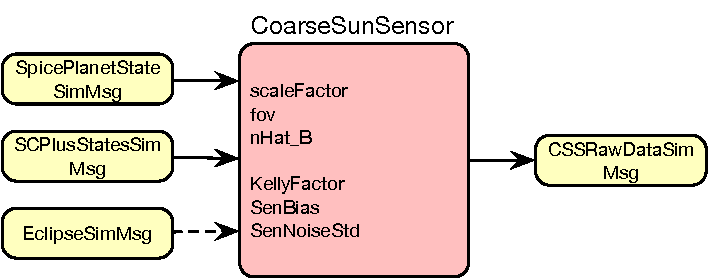
\includegraphics[]{Figures/moduleDiagram}
	}
	\caption{Illustration of the CoarseSunSensor() modulej}
	\label{fig:moduleDiagram}
\end{figure}
\section{Introduction}
This document describes how Coarse Sun Sensor (CSS) devices are modeled in the Basilisk software.  Each CSS is modeled through a nominal cosine response relative to the sunlight incidence angle.  This response can then be corrupted, or reduced due to being in a planet's shadow.  It is possible to add individual CSS sensors to the BSK evaluation stack.  However, it is typically simpler to use the {\tt CSSConstellation()} class to store a list of CSS units which are updated as a group, along with a unique CSS array output message.

\section{Single CSS module}
\subsection{I/O Messages}
First, let us discuss the input and output messages of the individual CSS sensor module.  The two required input messages are of the type {\tt SpicePlanetStateSimMsg} and {\tt SCPlusStatesSimMsg}.  The first message is used to determine the sun's location relative to the inertial frame $\leftexp{N}{\bm r}_{\sun/\mathcal{N}}$.  The second message is used to read in the spacecraft inertial position vector relative to the same inertial frame $\leftexp{N}{\bm r}_{\cal B/N}$.  Finally, the last message is optional.  If it is connected, it provides the sun shadow parameter indicating if the spacecraft is in a planet's shadow.  

The output message of an individual CSS unit creates a message containing the simulated CSS sensor.


\subsection{CSS Signal Simulation}
To evaluate the sun heading vector $\bm s$, the satellite and sun position vectors are used.
\begin{equation}
	\leftexp{N}{\bm s} = \leftexp{N}{\bm r}_{\sun/\mathcal{N}} - \leftexp{N}{\bm r}_{\cal B/N}
\end{equation}
After normalizing this vector to $\hat{\bm s}$ and mapping $\bm\sigma_{\cal B/N}$ to $[BN]$, it is mapped into body frame components through
\begin{equation}
	\leftexp{B}{\hat{\bm s}} = [BN] \leftexp{N}{\hat{\bm s}}
\end{equation}

The CSS sensor unit normal vector is given by $\leftexp{B}{\hat{\bm n}}$ in body frame components.  The normalized cosine sensor signal $\hat\gamma$ is thus determined through
\begin{equation}
	\hat \gamma = \hat{\bm n} \cdot \hat{\bm s} = \cos\phi
\end{equation}
where $\phi$ is the CSS sunlight incidence angle.  
This is the normalized CSS signal where 1 is returned if the sensor is looking straight at the sun.  If the sensor axis $\hat{\bm n}$ is more the field of view half-angle (set through {\tt fov}) from the sun axis, then a 0 signal is simulated.  This {\tt fov} variable is the angle from $\hat{\bm n}$ beyond which the CSS signal is set to zero.  

Let $p_{s}$ be the local solar shadow parameter.  If the spacecraft is outside of a planet's shadow, this value is 1.  If it is within the shadow, then it is $0\le p_{s} < 1$.  The shadow adjusted CSS signal is thus computed as 
\begin{equation}
	\hat{\gamma}_{s} = \hat{\gamma} p_{s}
\end{equation}

%Let $p_{a}$ be the CSS normalized contribution due to the planet's albedo value, then the final true CSS signal is 
%\begin{equation}
%	\hat\gamma_{\text{true}} = \hat{\gamma}_{s} + p_{a}
%\end{equation}

To simulate CSS signal corruptions, then a Kelly curve corruption, a bias and a gaussian noise can be included.  The normalized bias is set through {\tt SenBias}, while the normalized noise is set through {\tt SenNoiseStd}.   Let $\bm p_{n}$ be the normalized sensor noise.  Note that this noise levels is non-dimensional relative to the unit cosine curve.  

\begin{figure}[htb]
	\centerline{
	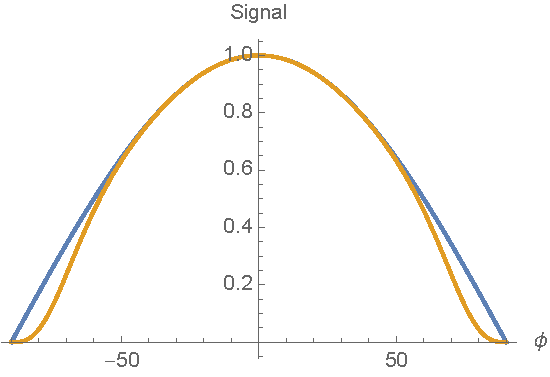
\includegraphics[]{Figures/kelly}
	}
	\caption{Kelly distortion illustration with $\kappa = 0.1$}
	\label{fig:kelly}
\end{figure}
The Kelly corruption parameter allows for the CSS signal to pinch towards zero for larger incidence angles as illustrated in Figure~\ref{fig:kelly}.  The amount of signal distortion is set through $\kappa$, where the Kelly factor $p_{\kappa}$ is then computed as 
\begin{equation}
	p_{\kappa} = 1 - e^{-\hat\gamma_{s}^{2}/\kappa}
\end{equation}
The corrupted normalized CSS signal is then
\begin{equation}
	\hat \gamma_{c} = (\hat\gamma_{s} + p_{a}) p_{\kappa} + p_{n}
\end{equation}

At this point the signal shape is correct, but not the scale.  The final step is to scale.  Using the {\tt scaleFactor} $=\alpha$ parameter, the CSS signal is now scaled to a dimensional value where the peak is not 1, but rather {\tt scaleFactor}.  
\begin{equation}
	\gamma = \hat{\gamma}_{c} \alpha
\end{equation}





\subsection{Setting the CSS Unit Direction Vector}



\subsection{Module Parameters}
This section describes the various module parameters that can be set via Python to configure the CSS unit.  The platform frame is 

\subsubsection{{\tt theta} Parameter}
This is the CSS azimuth angle relative to the platform frame.





\end{document}
